\documentclass{beamer}

\usepackage{graphicx,hyperref,fes,url}
\usepackage[english]{babel}
\usepackage[latin1]{inputenc}
%\usepackage{times}
\usepackage[T1]{fontenc}
\usepackage{multirow}
\usepackage{capt-of}
\usepackage{graphicx}
\usepackage{array}
\usepackage{tikz}
\usepackage{hyperref}


% The title of the presentation:
%  - first a short version which is visible at the bottom of each slide;
%  - second the full title shown on the title slide;
\title[FES style for Beamer]{
  UAlberta FES style for Beamer \LaTeX}

% Optional: a subtitle to be dispalyed on the title slide

% The author(s) of the presentation:
%  - again first a short version to be displayed at the bottom;
%  - next the full list of authors, which may include contact information;

\author[Author Short]{
  Pim Vullers MSc \and Martijn Sprengers \\\medskip
  {\small \url{p.vullers@cs.ru.nl} \and \url{m.sprengers@student.ru.nl}} \\
  {\small \url{http://www.cs.ru.nl/~pim/}}}

% The institute:
%  - to start the name of the university as displayed on the top of each slide
%    this can be adjusted such that you can also create a Dutch version
%  - next the institute information as displayed on the title slide
\institute[University of Alberta]{
  Future Energy Systems Symposium\\
  University of Alberta}

% Add a date and possibly the name of the event to the slides
%  - again first a short version to be shown at the bottom of each slide
%  - second the full date and event name for the title slide

\renewcommand{\(}{\begin{columns}}
\renewcommand{\)}{\end{columns}}
\newcommand{\<}[1]{\begin{column}{#1}}
\renewcommand{\>}{\end{column}}
%%%%%%%%%%%%%%%%%%%%%%%%%%%%%%%%%%%%%%%%%%%%%%%%%%





\newcommand{\degC}{$^o$C$\,$}
\newcommand{\co}{$\text{CO}_{2}\,$}
\newcommand{\tx}{$G_{2\times\text{CO}_2}$}
\newcommand{\Real}{\mathbb R}



% The main document



\begin{document}




\title{Carbon price pass through in electricity with known prices}
%\author{Branko Bo\v skovi\'{c} \and Andrew Leach \and Charles F.\ Mason}
%\institute{University of Alberta  \and University of Alberta  \and University of Wyoming}

%\author[shortname]{author1 \inst{1} \and author2 \inst{2}}
%\institute[shortinst]{\inst{1} affiliation for author1 \and %
 %                     \inst{2} affiliation for author2}

\author[Short Name (U ABC)]{%
  \texorpdfstring{%
    \begin{columns}
      \column{.1\linewidth}
      \column{.4\linewidth}
      \centering
      Andrew Leach \\University of Alberta
      \column{.4\linewidth}
      \centering
      Blake Shaffer \\University of Calgary
      \column{.1\linewidth}
      \end{columns}
 }
 {Leach and Shaffer (2022)}
}
\date{\small May, 2019}
\frame[plain]{
  \titlepage
}


\section{Introduction}
\begin{frame}{Carbon Pricing, Electricity Markets and Output-Based Allocations}
\vbox to \textheight{
  \begin{block}{}
    \begin{itemize}
    \item Impacts of carbon pricing has become a central policy question in Canada and globally
    \item Electricity markets, at least in certain jurisdictions are ideal environments in which to study responses to carbon prices
    \item Rich, hourly electricity market data allows us to observe firm-level decisions with respect to carbon price pass through
    \item Fabra and Reguant (2014) shows how firms respond to emissions credit prices and that lump-sum credit allocations were not distortionary in the short run
    \item Alberta policy changes alter both carbon prices and output-based credit allocations
    \item Brown et al. (2018) have looked at the dynamics of such a market in a simplified, simulation model
    \end{itemize}
  \end{block}
\vfill}
\end{frame}




%\begin{frame}{Oil sands reserves\hspace{3cm} \small Source: AER (2013)}
%\pgfputat{\pgfxy(0,.25)}{\pgfimage[width=4.25in]{AB_reserves.pdf}}
%\end{frame}

\begin{frame}{Alberta's Power Market is an Ideal Laboratory}
\vbox to \textheight{
  \begin{block}{Alberta's power market:}
    \begin{itemize}
    \item Alberta's power market is relatively small, isolated, and features a mix of generation technologies
    \item Our peak internal load for 2018 was 11,697 MW, while our lowest observed internal load was 	7,819 MW
    \item We have relatively minimal intertie capacity.  Alberta is connected to WECC (1325 MW export and 1500 MW import path-rating) via Montana and BC) and to Saskatchewan (150 MW path-rating) but significant hourly variability in capacity which helps us with identification
    \item Supply mix (2018) was 44.8\% coal, 21.1\% net-to-grid from combined heat and power plants, 18.5\% natural gas, 2.9\% hydro, 6.4\% wind, 	1.0\% other sources including solar and 5.2\% imports.
  \end{itemize}
  \end{block}
\vfill}
\end{frame}

\begin{frame}{Alberta's Policy Changes as Treatments}
\vbox to \textheight{
  \begin{block}{Alberta's GHG policy changes:}
    \begin{itemize}
    \item From 2007 to 2015, Alberta's \textit{Specified Gas Emitters Regulation} imposed a carbon price of \$15 per tonne with output-based allocations at a rate of 88\% of a facility's historic emissions intensity if the facility's annual emissions were more than 100,000 tonnes per year
    \item In 2015, these parameters were changed to \$20 per tonne with allocations equal to 85\% of historic emissions intensities in 2016 and \$30 per tonne with allocations of 80\% in 2017.
    \item 2007-2017 system also had generous emissions credits for combined heat and power systems
    \item In 2018, the system changed again, to one with output-based allocations fixed for all generators (0.37t/MWh) including for net generation from combined heat and power.
    \end{itemize}
  \end{block}
\vfill}
\end{frame}


\begin{frame}{Data Richness}
\vbox to \textheight{
  \begin{block}{We have data on:}
    \begin{itemize}
    \item Hourly merit order (power offers) by unit with data on who held offer control for that unit at that time
    \item Hourly forecast and actual loads and prices
    \item Hourly weather for Edmonton, Calgary, and Fort McMurray
    \item Hourly imports, exports, and intertie capabilities
    \item Hourly wind forecasts including 3 and 7 day advanced forecasts.
    \item Plant-level emissions intensities and historic allocation rates under \textit{SGER}
    \end{itemize}
  \end{block}
\vfill}
\end{frame}





\section{Results Preview}
\begin{frame}{Carbon pricing impacts on power markets}
\vbox to \textheight{
  \begin{block}{Our results show that:}
    \begin{itemize}
    \item ...
    \end{itemize}
  \end{block}
\vfill}
\end{frame}


\begin{frame}{Carbon Pricing Policy and Power Generation Sources}
   \tikz [remember picture,overlay]
    \node[yshift=-.5cm,xshift=0cm] at (current page.center)
       {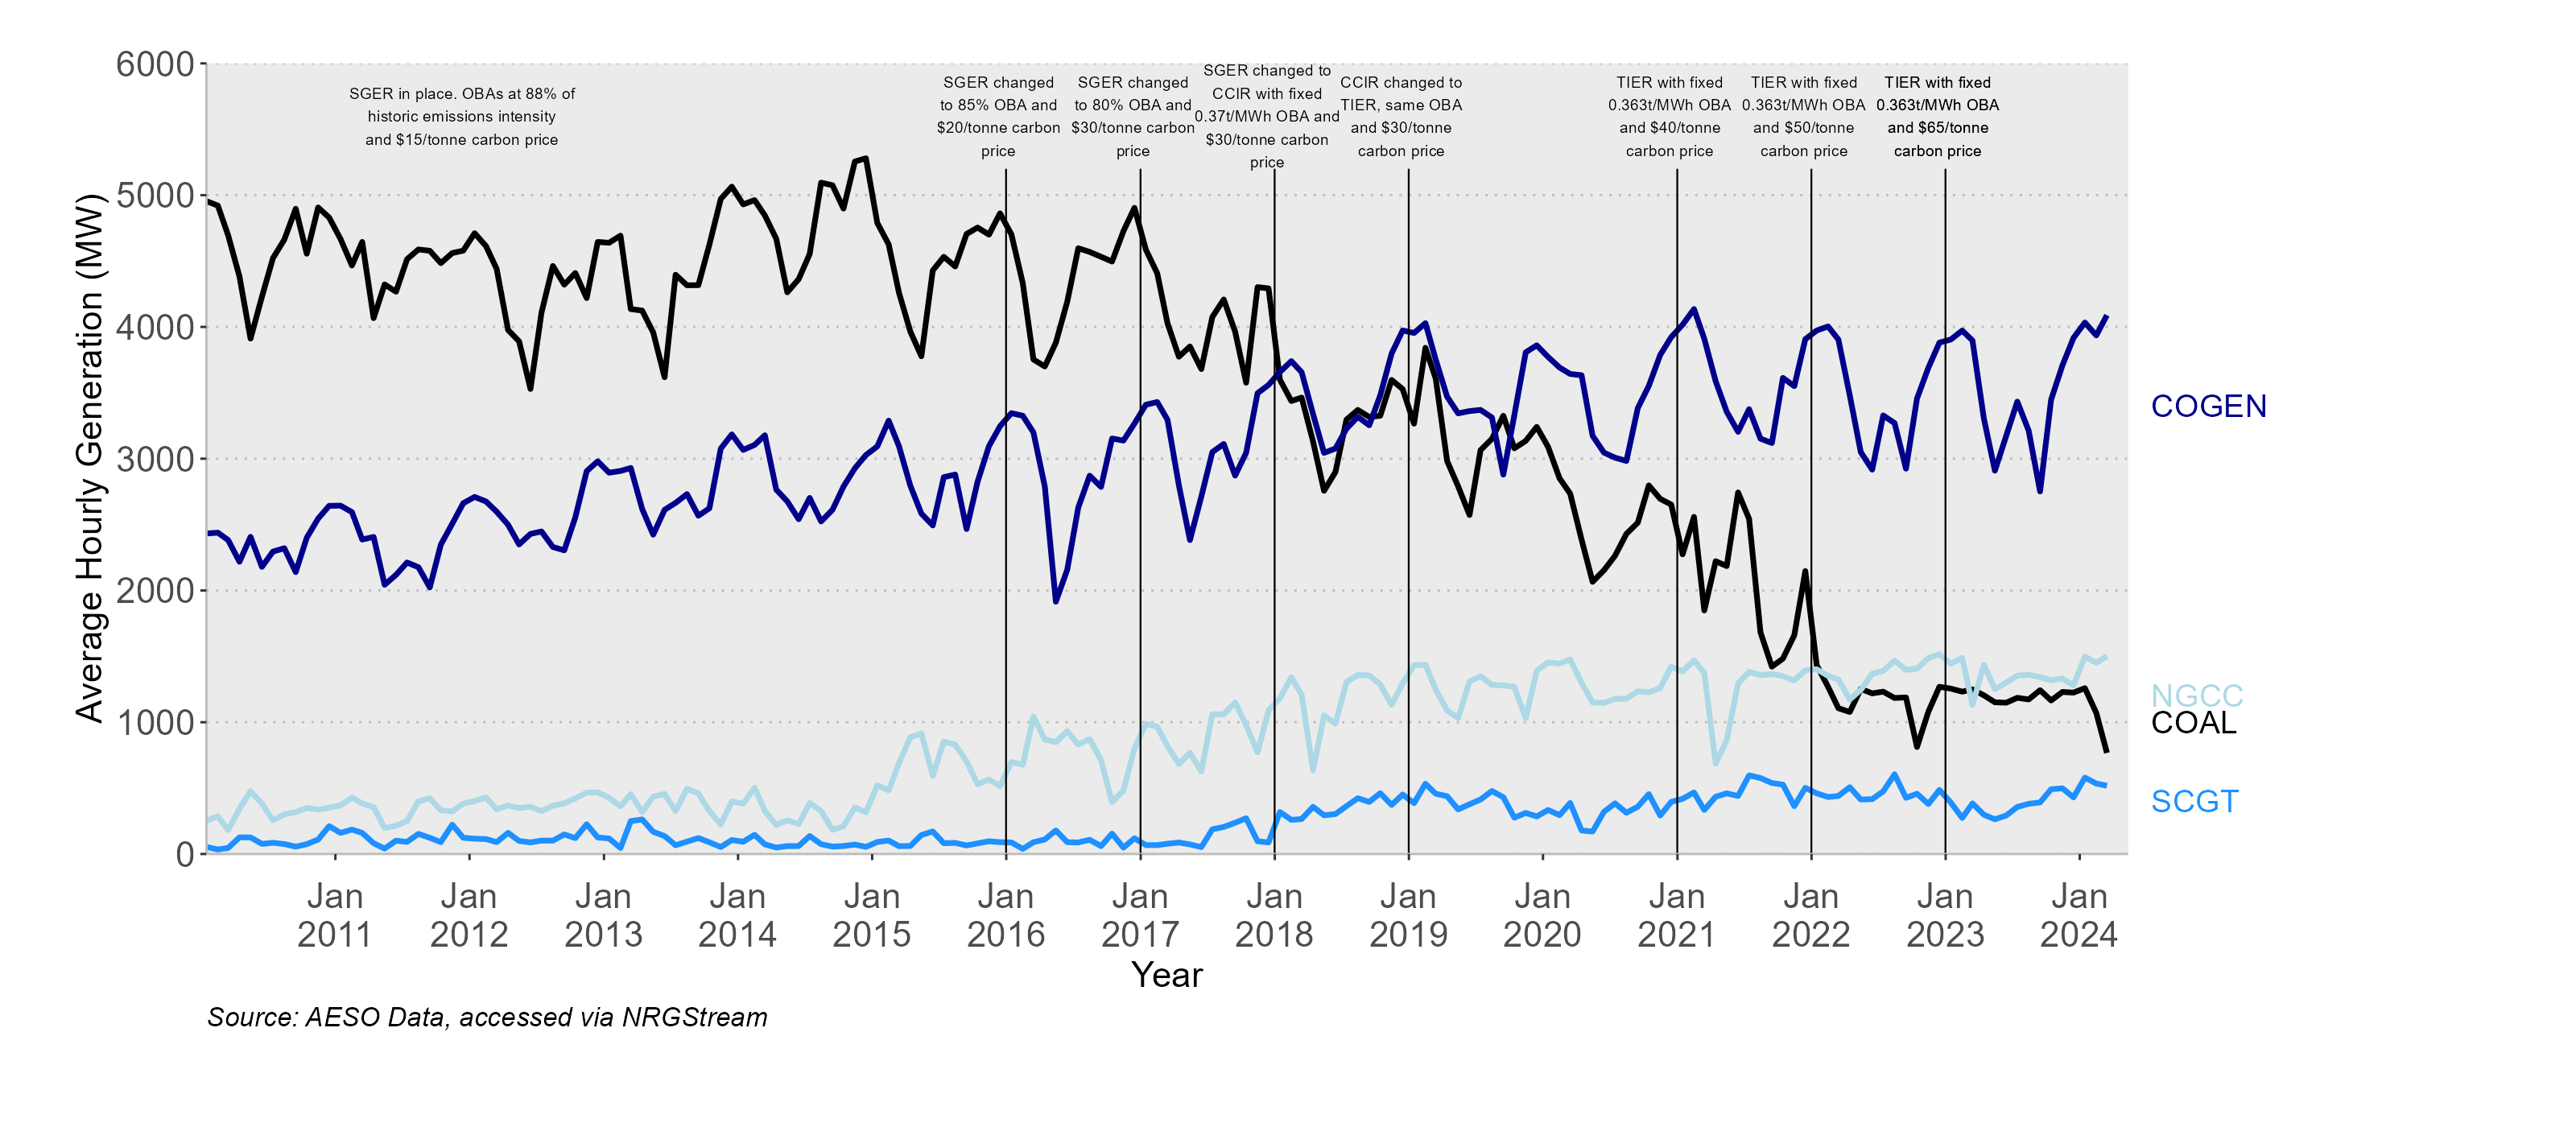
\includegraphics[width=.9\paperwidth]{../../alberta_power/gen_ghg_price.png}}; \vspace{1cm}
   \vfill
\end{frame}


\begin{frame}{Carbon Intensity of Alberta Power}
   \tikz [remember picture,overlay]
    \node[yshift=-.5cm,xshift=0cm] at (current page.center)
       {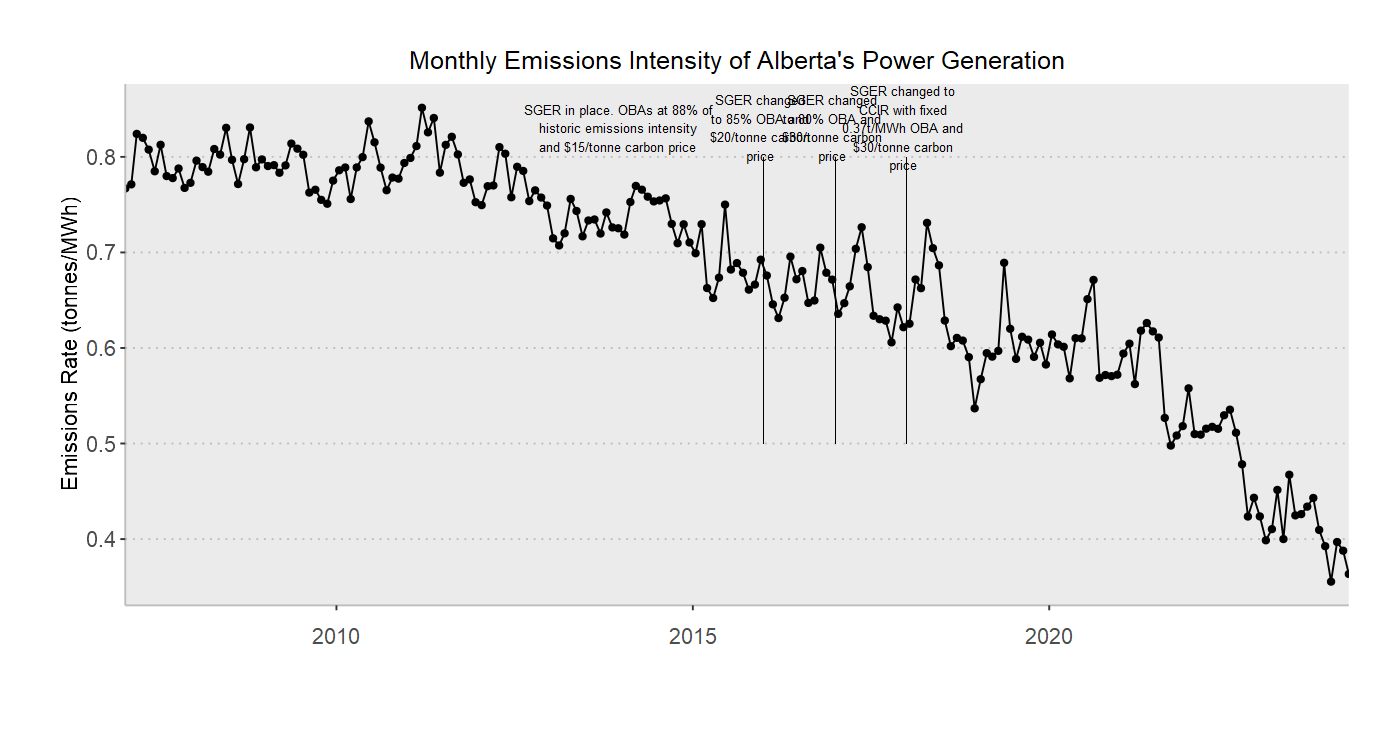
\includegraphics[width=.9\paperwidth]{../../alberta_power/monthly_ghg_mwh.png}}; \vspace{1cm}
   \vfill
\end{frame}



\begin{frame}{Carbon pricing policy impacts on the merit order}
   %\tikz [remember picture,overlay]
   %# \node[yshift=-.5cm,xshift=0cm] at (current page.center)
    %    #{\includegraphics[width=.9\paperwidth]{tax_runs.png}}; \vspace{1cm}
   \vfill
\end{frame}


\begin{frame}{Within-group, plant-level impacts of policies}
   %\tikz [remember picture,overlay]
   %# \node[yshift=-.5cm,xshift=0cm] at (current page.center)
    %    #{\includegraphics[width=.9\paperwidth]{tax_runs.png}}; \vspace{1cm}
   \vfill
\end{frame}


\section{Empirical Framework}
\begin{frame}{Empirical Framework}
    \begin{block}{}
    \begin{itemize}
    \item The goal of our empirical framework is to estimate the degree to which carbon prices pass through to merit order behaviour and thus to electricity prices
    \item We follow Fabra and Reguant (2014) which estimates:
    \begin{eqnarray*}\label{eq:production}
    \underset{\color{blue}\substack{\text{Cost}\\{\text{pass-through}}}} {p_{th}} &=&\underset{\color{blue}\substack{\text{Effect of GHG}\\{\text{price times rate}}}} {\rho\tau_te_{th}}
    +\underset{\color{blue}\substack{\text{Supply, demand and common}\\{\text{factor adjustments}}}} {\beta_0X_{th}+\beta_1X_{th}^D+\beta+2X_{th}^S}\\&+&
    \underset{\color{blue}\substack{\text{Fixed}\\{\text{effects}}}}{B_3I_{th}}
    + \underset{\color{blue}\substack{\text{Error}\\{\text{term}}}}{\epsilon_{th}}
    \end{eqnarray*}
    \item Alberta policy changes alter both carbon prices and output-based credit allocations over time, which changes the empirical specifications in our case slightly
    \item We have hourly forecast prices and loads (3 hour leads) which we can use as supply and demand indicators
    \item We also have both forecast and actual temperature and wind generation data over the sample time period
    \end{itemize}
  \end{block}
   \vfill
\end{frame}



\section{Empirical Framework}
\begin{frame}{Empirical Framework}
    \begin{block}{}
    \begin{itemize}
    \item Like Fabra and Reguant, we also have hourly bids by plant for up to 7 blocks - an individual supply function - which we can then use to estimate firm-level residual demand for the marginal producer
    \begin{eqnarray*}\label{eq:production}
    \underset{\color{blue}\substack{\text{Marginal bid of firm $i$}\\{\text{unit $j$, time $th$}}}} {b_{ijth}} &=&\underset{\color{blue}\substack{\text{Effect of GHG}\\{\text{price times rate}}}} {\gamma\tau_te_{j}}
    +\underset{\color{blue}\substack{\text{Marginal cost}\\{\text{estimates}}}} {\beta c_{jt}}\\&+&
    \underset{\color{blue}\substack{\text{Approximate}\\{\text{markup}}}}{\theta\hat{m}_{ijth}}
    + \underset{\color{blue}\substack{\text{Error}\\{\text{term}}}}{\epsilon_{ijth}}
    \end{eqnarray*}
\item in our case, emissions prices vary over time as do allocation rates, so we need to modify both structures
    \end{itemize}
  \end{block}
   \vfill
\end{frame}



\section{Results}

\begin{frame}{Results}
   %\tikz [remember picture,overlay]
   %# \node[yshift=-.5cm,xshift=0cm] at (current page.center)
    %    #{\includegraphics[width=.9\paperwidth]{tax_runs.png}}; \vspace{1cm}
   \vfill
\end{frame}


\section{Discussion}

\begin{frame}{Discussion}
   %\tikz [remember picture,overlay]
   %# \node[yshift=-.5cm,xshift=0cm] at (current page.center)
    %    #{\includegraphics[width=.9\paperwidth]{tax_runs.png}}; \vspace{1cm}
   \vfill
\end{frame}


\section{Other FES Theme 06 Research}
\begin{frame} Secanell group
\begin{block}{}
\footnotesize{\begin{itemize}
  \item Design, procurement and installation of low and high temperature electrolysis fabrication and testing facilities
  \item Fabrication of single-cell low temperature electrolyzer prototypes using iridium and iridium oxide catalysts
  \item Demonstrated, for the first time, the use of inkjet printing as a feasible technology to fabricate low temperature electrolyzer cells  (https://doi.org/10.1149/2.1101807jes)
   \item Development of a novel nano-pompon-like iridium catalyst superstructure for low temperature fuel cell electrolyzers (https://doi.org/10.1016/j.jcat.2019.01.018)
   \item Development of a novel technique for characterization of iridium catalyst degradation (https://doi.org/10.1016/j.jcat.2019.01.018)
 \item Development of novel micro-structures for high temperature solid oxide electrolyzers and fuel cells (https://doi.org/10.1016/j.electacta.2018.02.055)
  \end{itemize}}
The project currently involves 5 PhD students and 1 MSc, 5 faculty (1 in MECE, 3 in CHEME and 1 in Chem). We are also collaborating with Ionomr, a firm in BC (https://ionomr.com/).
  \end{block}
   \vfill
\end{frame}



\begin{frame}{Secanell Group}
   \tikz [remember picture,overlay]
    \node[yshift=-.5cm,xshift=0cm] at (current page.center)
      {\includegraphics[height=3in]{../../secanell_1}}; \vspace{1cm}
   \vfill
\end{frame}

\section{Other FES Theme 06 Research}
\begin{frame} Secanell group
\begin{block}{}
\footnotesize{\begin{itemize}
  \item Design, procurement and installation of low and high temperature electrolysis fabrication and testing facilities
  \item Fabrication of single-cell low temperature electrolyzer prototypes using iridium and iridium oxide catalysts
  \item Demonstrated, for the first time, the use of inkjet printing as a feasible technology to fabricate low temperature electrolyzer cells  (https://doi.org/10.1149/2.1101807jes)
   \item Development of a novel nano-pompon-like iridium catalyst superstructure for low temperature fuel cell electrolyzers (https://doi.org/10.1016/j.jcat.2019.01.018)
   \item Development of a novel technique for characterization of iridium catalyst degradation (https://doi.org/10.1016/j.jcat.2019.01.018)
 \item Development of novel micro-structures for high temperature solid oxide electrolyzers and fuel cells (https://doi.org/10.1016/j.electacta.2018.02.055)
  \end{itemize}}
The project currently involves 5 PhD students and 1 MSc, 5 faculty (1 in MECE, 3 in CHEME and 1 in Chem). We are also collaborating with Ionomr, a firm in BC (https://ionomr.com/).
  \end{block}
   \vfill
\end{frame}


\begin{frame}{Secanell Group}
   \tikz [remember picture,overlay]
    \node[yshift=-.5cm,xshift=0cm] at (current page.center)
      {\includegraphics[height=3in]{../../secanell_2}}; \vspace{1cm}
   \vfill
\end{frame}


\section{Other FES Theme 06 Research}
\begin{frame} Secanell group
\begin{block}{}
\footnotesize{\begin{itemize}
  \item Design, procurement and installation of low and high temperature electrolysis fabrication and testing facilities
  \item Fabrication of single-cell low temperature electrolyzer prototypes using iridium and iridium oxide catalysts
  \item Demonstrated, for the first time, the use of inkjet printing as a feasible technology to fabricate low temperature electrolyzer cells  (https://doi.org/10.1149/2.1101807jes)
   \item Development of a novel nano-pompon-like iridium catalyst superstructure for low temperature fuel cell electrolyzers (https://doi.org/10.1016/j.jcat.2019.01.018)
   \item Development of a novel technique for characterization of iridium catalyst degradation (https://doi.org/10.1016/j.jcat.2019.01.018)
 \item Development of novel micro-structures for high temperature solid oxide electrolyzers and fuel cells (https://doi.org/10.1016/j.electacta.2018.02.055)
  \end{itemize}}
The project currently involves 5 PhD students and 1 MSc, 5 faculty (1 in MECE, 3 in CHEME and 1 in Chem). We are also collaborating with Ionomr, a firm in BC (https://ionomr.com/).
  \end{block}
   \vfill
\end{frame}

\begin{frame}{Secanell Group}
   \tikz [remember picture,overlay]
    \node[yshift=-.5cm,xshift=0cm] at (current page.center)
      {\includegraphics[width=4.5in]{../../secanell_3}}; \vspace{1cm}
   \vfill
\end{frame}

\section{Other FES Theme 06 Research}
\begin{frame} Secanell group
\begin{block}{}
\footnotesize{\begin{itemize}
  \item Design, procurement and installation of low and high temperature electrolysis fabrication and testing facilities
  \item Fabrication of single-cell low temperature electrolyzer prototypes using iridium and iridium oxide catalysts
  \item Demonstrated, for the first time, the use of inkjet printing as a feasible technology to fabricate low temperature electrolyzer cells  (https://doi.org/10.1149/2.1101807jes)
   \item Development of a novel nano-pompon-like iridium catalyst superstructure for low temperature fuel cell electrolyzers (https://doi.org/10.1016/j.jcat.2019.01.018)
   \item Development of a novel technique for characterization of iridium catalyst degradation (https://doi.org/10.1016/j.jcat.2019.01.018)
 \item Development of novel micro-structures for high temperature solid oxide electrolyzers and fuel cells (https://doi.org/10.1016/j.electacta.2018.02.055)
  \end{itemize}}
The project currently involves 5 PhD students and 1 MSc, 5 faculty (1 in MECE, 3 in CHEME and 1 in Chem). We are also collaborating with Ionomr, a firm in BC (https://ionomr.com/).
  \end{block}
   \vfill
\end{frame}


\section{Other FES Theme 06 Research}
\begin{frame} Secanell group
\footnotesize{\begin{itemize}
  \item Design, procurement and installation of low and high temperature electrolysis fabrication and testing facilities
  \item Fabrication of single-cell low temperature electrolyzer prototypes using iridium and iridium oxide catalysts
  \item Demonstrated, for the first time, the use of inkjet printing as a feasible technology to fabricate low temperature electrolyzer cells  (https://doi.org/10.1149/2.1101807jes)
   \item Development of a novel nano-pompon-like iridium catalyst superstructure for low temperature fuel cell electrolyzers (https://doi.org/10.1016/j.jcat.2019.01.018)
   \item Development of a novel technique for characterization of iridium catalyst degradation (https://doi.org/10.1016/j.jcat.2019.01.018)
 \item Development of novel micro-structures for high temperature solid oxide electrolyzers and fuel cells (https://doi.org/10.1016/j.electacta.2018.02.055)
  \end{itemize}}
The project currently involves 5 PhD students and 1 MSc, 5 faculty (1 in MECE, 3 in CHEME and 1 in Chem). We are also collaborating with Ionomr, a firm in BC (https://ionomr.com/).
   \vfill
\end{frame}



\begin{frame}{Contact info}
\begin{center}
Andrew Leach\bigskip \\
School of Business, University of Alberta\bigskip \\
Email: \href{mailto:aleach@ualberta.ca}{andrew.leach@ualberta.ca}\bigskip \\
Twitter: \href{http://twitter.com/andrew_leach}{\url{@andrew_leach}}
\end{center}
\vfill
\end{frame}


\end{document} 